\subsection{Implementación SRGAN.}

La implementación de este modelo se realizara utilizando la arquitectura presentada
en \cite{SRGAN} mediante el lenguaje \emph{Python} utilizando la librería de alto nivel \emph{Keras}

Keras es una API que proporciona numerosos bloques
de construcción útiles los cuales pueden ser conectados para crear arquitecturas de
aprendizaje profundo altamente complejas.

Para el entrenamiento de las redes, Keras utiliza una de las tres librerías como
\emph{backend} para este propósito: \emph{TensorFlow}, \emph{CNTK}, o \emph{Theano}. Para esta implementación
se utiliza \emph{TensorFlow}, que es una librería de Python de código abierto para el
aprendizaje automático, esta fue desarrollada por Google.

Utilizaremos el dataset MIRFLICKR \cite{MIRFLICKR} el cual es una base de datos de imágenes
extraídas de la red social flickr, esta base consta de 25000 imágenes y la principal ventaja es 
que las imágenes son muy variadas por lo cual es ideal en el entrenamiento de una red neuronal capaz 
de mejorar los detalles de una imagen. Cabe resaltar que no se utilizaron todas las imágenes del dataset
debido al tiempo de ejecución del entrenamiento, así como las limitantes de hardware al ejecutar el código.



\subsubsection{Modelo generador.}

Las imágenes originales del dataset son de una dimensión de 500x500 pixeles, para el modelo generador
se utiliza una imagen de entrada de baja resolución de 32x32 pixeles y la imagen de alta resolución de salida
será de 128x128 pixeles, teniendo un escalado de 4 veces el tamaño original, algunas de estas imágenes pueden
visualizarse en la imagen \ref{fig:fr_dataset}.






\begin{figure}[H]
  \begin{center}
    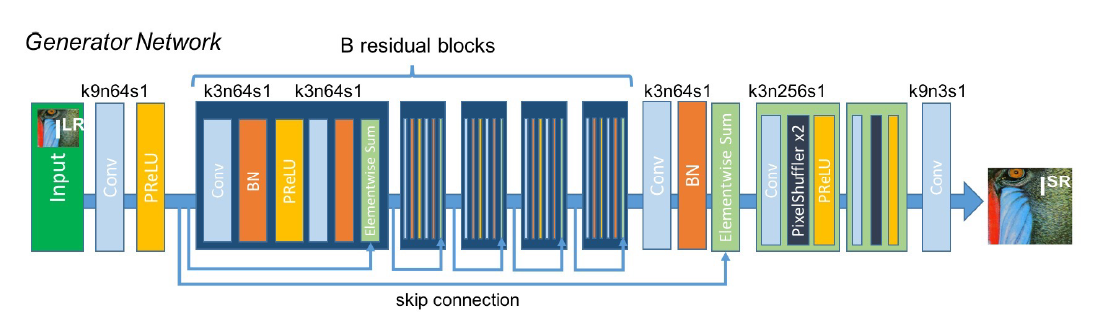
\includegraphics[scale = 0.7]{Imp_generador.png}
    \caption{Arquitectura del generador de la SRGAN,\emph{k} es el tamaño del
    filtro, \emph{n} es la dimensión del mapa de características (capa de convolución) y \emph{s} indica
    el valor del parámetro stride. Imagen tomada de \cite{SRGAN}}
    \label{Alexis4}
  \end{center}
\end{figure}

\subsubsection{Modelo discriminador.}

\begin{figure}[H]
  \begin{center}
    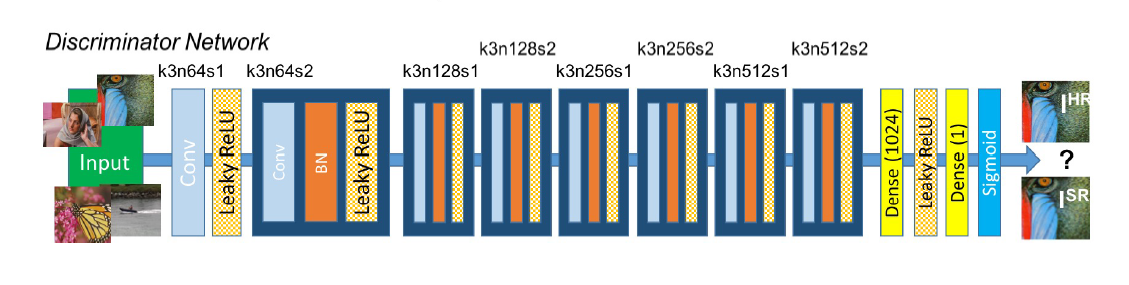
\includegraphics[scale = 0.7]{Imp_discriminador.png}
    \caption{Arquitectura del Discriminador de la SRGAN, \emph{k} es el tamaño
    del filtro, \emph{n} es la dimensión del mapa de características (capa de convolución) y \emph{s}
    indica el valor del parámetro stride. Imagen tomada de \cite{SRGAN}}
    \label{Alexis5}
  \end{center}
\end{figure}

\subsubsection{Entrenamiento}

EL modelo de entrenamiento de las GAN´s como se ha mencionado en \cite{GANs} y \cite{SRGAN}, es un proceso en el cual
los dos modelos compiten, el generador por engañar al discriminador y el discriminador por no permitirlo, en la figura \ref{Alexis6}
podemos ver el proceso en el cual se basa el entrenamiento.

\begin{figure}[H]
    \begin{center}
      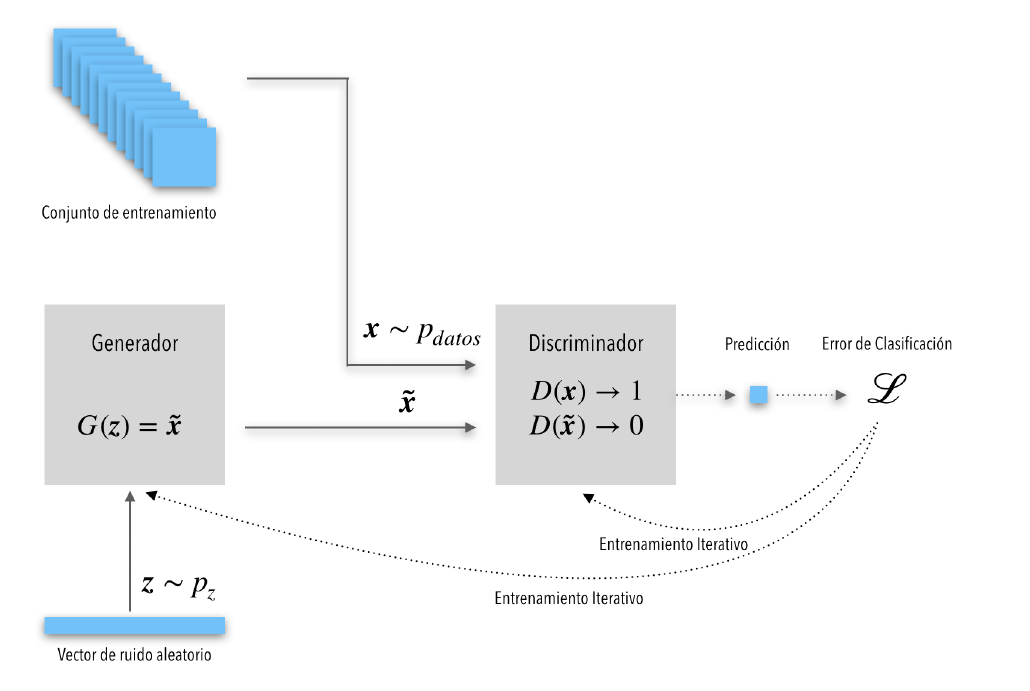
\includegraphics[scale = 0.6]{proceso_gan.png}
      \caption{Proceso de entrenamiento}
      \label{Alexis6}
    \end{center}
\end{figure}


Después de realizar las épocas de entrenamiento se puede apreciar que a mayor numero de imágenes y 
épocas los resultados suelen ser mejores sobre todo para imágenes que no están en el dataset,en la imagen
\ref{Alexis7} podemos observar la mejora que se obtiene con 200 épocas de entrenamiento para tan solo 13 imágenes 
aun así la reconstrucción es buena y se logran percibir algunos detalles.

\begin{figure}[H]
  \begin{center}
    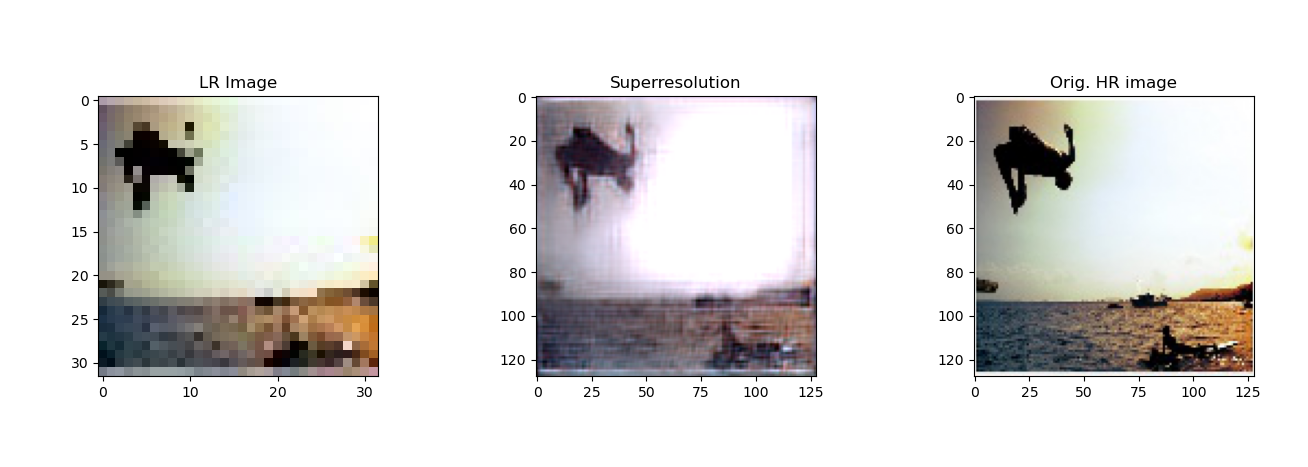
\includegraphics[scale = 0.4]{13im_200E.png}
    \caption{Imagen obtenida de un modelo generador de 200 épocas y 13 imágenes.}
    \label{Alexis7}
  \end{center}
\end{figure}

Conforme se aumentan las épocas de entrenamiento y el número de imágenes se comprueba
que los resultados son mejores como se observa en la imagen \ref{Alexis8} donde se aumentan
las épocas a 400 y el numero de imágenes a 50, con lo que podemos obtener mas detalles en nuestro modelo
gracias a al diversidad en estas imágenes.

\begin{figure}[H]
  \begin{center}
    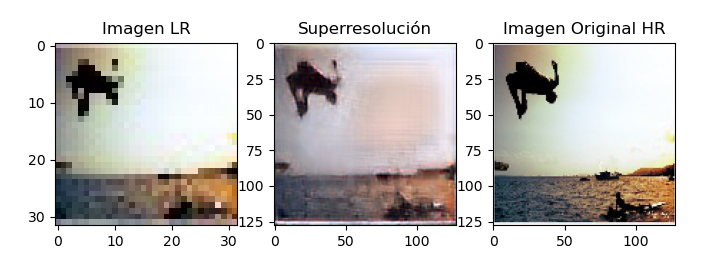
\includegraphics[scale = 0.9]{50im_400E.png}
    \caption{Imagen obtenida de un modelo generador de 400 épocas y 50 imágenes.}
    \label{Alexis8}
  \end{center}
\end{figure}

Una solución a este problema es realizar la carga del modelo generador antes del entrenamiento,
con esto el modelo generador toma la configuración de pesos y métricas anteriores y realiza el entrenamiento
a partir de estas, esto puede generar una mejora como se observa en la imagen \ref{Alexis9}, pero
también puede causar distorsión en el modelo que obtengamos como resultado, dada la interpretación del generador,
incluso se puede aumentar la perdida.

\begin{figure}[H]
  \begin{center}
    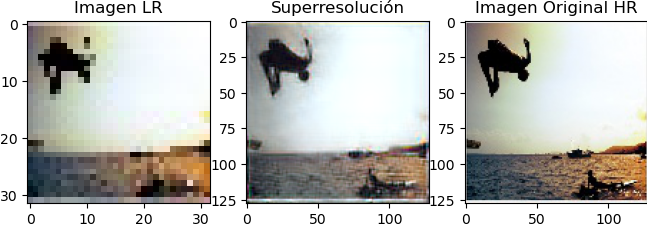
\includegraphics[scale = 0.57]{1000im_5E_Reentrenado.png}
    \caption{Imagen obtenida de un modelo generador entrenado a partir de 400 épocas y 50 imágenes cargado
    en el programa y luego entrenado a 5 épocas y 1000 imágenes.}
    \label{Alexis9}
  \end{center}
\end{figure}




\subsubsection{Métricas}

 Durante el entrenamiento podemos observar el tiempo que tarda nuestra red en realizar el entrenamiento, aunado a eso 
 podemos medir las perdidas de los modelos, dados los antecedentes, se tiene que las perdidas nos relacionan la mejora de la imagen
 a menor valor de perdida exista, mejor será la calidad del modelo generador, para el modelo discriminador ocurre lo mismo,
 entre menor sea el número, mejor podrá discernir entre una imagen generada y una real.

 Finalmente se puede observar que la Precisión del modelo generador tiende a un valor de 1,(100\%) esto quiere decir que
 en esa época sabrá discernir perfectamente una imagen de la otra, forzando al generador a tener menos perdida. Esto puede observarse en las
 gráficas de la imagen \ref{Alexis10}.

 \begin{table}[H]
  \centering
  \caption{Resultados Máximo y Mínimos de las perdidas.}
  \begin{tabular}{|l|l|l|}
  \hline
  \textbf{Criterio} & \textbf{Valor Máximo} & \textbf{Valor Mínimo}  \\ \hline
  Pérdida del Generador           & 228.5551261019351              & 23.898190839255033     \\
  Pérdida del Discriminador       & 1.236285184701566              & 1.6890162633455543e-16  \\
  Precisión Discriminador         & 1.0                            & 0.8630597014925373       \\ \hline
  \end{tabular}
\end{table}



\begin{figure}[H]
  \begin{center}
    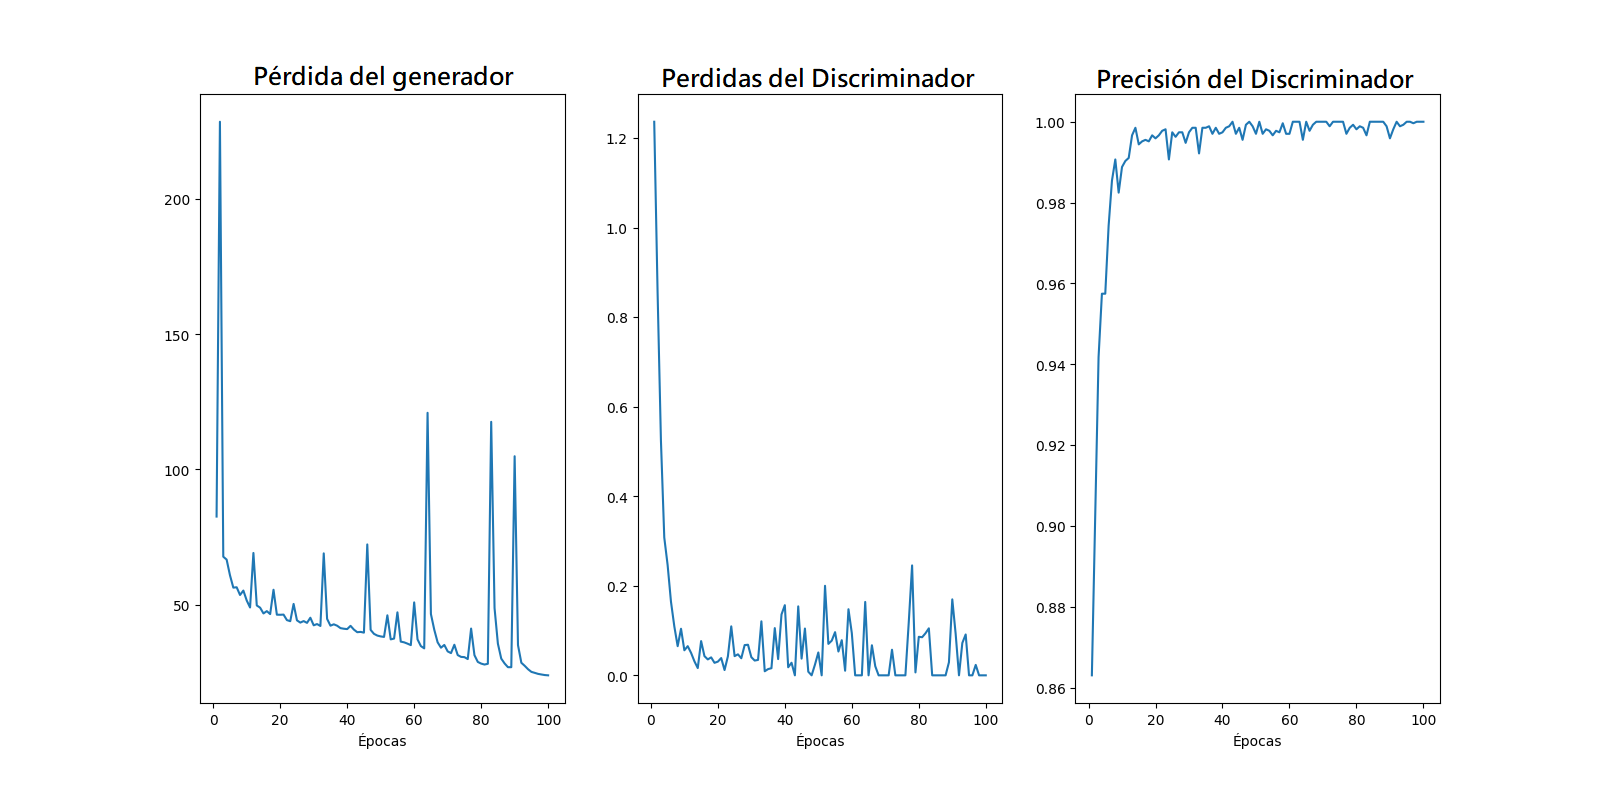
\includegraphics[scale = 0.6]{Graficasperdidas.png}
    \caption{Resultados de las perdidas durante el entrenamiento (2000 imágenes, 100 épocas)}
    \label{Alexis10}
  \end{center}
\end{figure}